% -----------------------------------------------
% DCC831 - TP Final: Geração de Piano Pop Condicionada por Emoção com
%                    Classifier-Free Guidance. UFMG 2026/2

% Requirements :
% * 6+n page length maximum
% * 10MB maximum file size
% * Copyright note must appear in the bottom left corner of first page
% (see conference website for additional details)
% -----------------------------------------------

\documentclass{article}
\usepackage[T1]{fontenc}
\usepackage[utf8]{inputenc}
\usepackage[brazilian]{babel}
\usepackage{ismir}
\usepackage{amsmath,cite,url}
\usepackage{graphicx}
\usepackage{color}

\graphicspath{{figures/}{../results/figures/}}

% Title. Please use IEEE-compliant title case when specifying the title here,
% as it has implications for the copyright notice
% ------
\title{Geração de Piano Pop Condicionada por Emoção com Classifier-Free Guidance}

% Note: Please do NOT use \thanks or a \footnote in any of the author markup

\multauthor
  {Cecilia J. V. M. Pereira \hspace{1cm} Daniel Barreto Torres}
  {{\bf Erick Soares de Souza \hspace{1cm} Felipe Lopes Gomide}\\
  {\bf Leonardo Romano Andrade \hspace{1cm} Lucas Junqueira Carvalhido}\\
  Universidade Federal de Minas Gerais, Brazil\\
  {\tt\small ceciliajunq@ufmg.br, daniboybt@ufmg.br, ericksoares@ufmg.br,}\\
  {\tt\small fgomide@ufmg.br, leo-romano@ufmg.br, lucasjc@ufmg.br}
  }

% For the author list in the Creative Common license, please enter author names.
% Please abbreviate the first names of authors and add 'and' between the second to last and last authors.
\def\authorname{C. Pereira, D. Torres, E. Souza, F. Gomide, L. Andrade, and L. Carvalhido}

% ismir.sty fixa "ABSTRACT" em inglês; mantém o resumo em português (como no TP1)
\renewcommand{\abstract}{\begin{center}\bf RESUMO\end{center}}
\renewcommand{\tablename}{Tabela}
\renewcommand{\figurename}{Figura}
% ismir.sty fixa "References" em inglês; mesma definição, com o título em português
\def\thebibliography#1{
  \section{Referências}\list
  {[\arabic{enumi}]}{
  \settowidth\labelwidth{[#1]}\leftmargin 1em
  \advance\leftmargin\labelsep
  \usecounter{enumi}
  }
  \def\newblock{\hskip .01em plus .01em minus .01em}
  \sloppy\clubpenalty4000\widowpenalty4000
  \sfcode`\.=1000\relax
}

% Optional: To use hyperref, uncomment the following.
\usepackage[bookmarks=false,pdfauthor={\authorname},pdfsubject={\pdfsubject},hidelinks]{hyperref}
% Mind the bookmarks=false option; bookmarks are incompatible with ismir.sty.

\sloppy % please retain sloppy command for improved formatting

\begin{document}

\maketitle

\begin{abstract}
  Este trabalho investiga a geração de trechos de piano pop condicionados a um
  dos quatro quadrantes emocionais do modelo de Russell. Um Transformer decoder
  é pré-treinado no Pop1k7 e ajustado no EMOPIA+ com um token de emoção que,
  durante o ajuste fino, é trocado aleatoriamente por um token nulo, o que
  permite aplicar \emph{classifier-free guidance} (CFG) apenas na amostragem,
  sem retreinar o modelo. O sistema é comparado a uma LSTM e a uma cadeia de
  Markov quanto à aderência à emoção, à qualidade e à diversidade. Os resultados
  mostram que o CFG aumenta bastante a aderência sem perda de qualidade. O
  ganho, no entanto, vem quase todo do arousal, enquanto a valência praticamente
  não muda, pois o modo maior ou menor das peças geradas não distingue os
  quadrantes. O código está disponível em
  \url{https://github.com/Lucas-Junqueira/TP-Final-de-IA-pra-Musica}.
\end{abstract}

% -----------------------------------------------
\section{Introdução}\label{sec:intro}

A geração de música simbólica com redes neurais avançou rapidamente com os
Transformers autoregressivos, hoje capazes de produzir piano expressivo com
estrutura métrica coerente~\cite{Huang2019:musictransformer,Huang2020:remi}.
Para servirem como ferramenta de composição, esses modelos também precisam
aceitar controles de alto nível, e a emoção é um dos mais naturais para quem
compõe ou escuta. Aqui, a emoção é descrita pelos quatro quadrantes do modelo
circumplexo de Russell~\cite{Russell1980:circumplex}, que combina valência
(positiva ou negativa) e arousal (alta ou baixa energia): Q1 (feliz), Q2
(tensa), Q3 (triste) e Q4 (calma). A tarefa é gerar trechos de piano pop
condicionados a um desses quadrantes.

A forma mais comum de condicionar a geração é inserir um token de emoção na
sequência e ajustar o modelo em dados rotulados. Hung et al.
(2021)~\cite{Hung2021:emopia} mostram que as peças geradas dessa forma obtêm
acurácia bem menor em um classificador de emoção do que as peças reais, o que
sugere que elas não carregam a emoção pedida ou se afastam demais das peças
reais para o classificador. O mesmo se observa no Transformer avaliado, que, com
condicionamento simples, acerta o quadrante pretendido em apenas 34\,\% das
amostras, segundo o classificador de emoção usado na avaliação.

Para reforçar a condição sem retreinar o modelo, aplica-se o
\emph{classifier-free guidance} (CFG) aos \emph{logits} de cada token, como
Sanchez et al. (2024)~\cite{Sanchez2024:cfg} fazem em modelos de linguagem.
Durante o ajuste fino, o token de emoção é trocado aleatoriamente por um token
reservado sem emoção, \texttt{<NULL>}, o mesmo usado em todo o pré-treino, de
modo que o mesmo modelo aprende a gerar com e sem a condição. Na amostragem, as
duas predições são combinadas a cada passo com um peso $\gamma$. Com
$\gamma = 1$, recupera-se o condicionamento simples, e com $\gamma > 1$ a
predição é extrapolada na direção da emoção pedida.

Investiga-se, então, quanto o CFG aumenta a aderência à emoção, qual o custo em
qualidade e diversidade, e se o efeito é diferente para valência e arousal. Os
resultados mostram que o CFG aproxima a aderência do teto do classificador sem
perda de qualidade, mas o ganho vem quase todo do arousal. A valência
praticamente não muda, pois o modo maior ou menor das peças geradas não
distingue os quadrantes em nenhum valor de $\gamma$.

A principal contribuição deste trabalho é mostrar que o CFG, já usado em modelos
de linguagem, também reforça o condicionamento por emoção na geração simbólica,
sem custo de treino além do descarte aleatório da condição. Um Transformer
decoder pré-treinado no Pop1k7 e ajustado no EMOPIA+ é avaliado em uma varredura
de $\gamma$ entre 1 e 10 e comparado a uma LSTM e a uma cadeia de Markov. Outra
contribuição é uma análise de atributos musicais das peças geradas, como
densidade de notas, intensidade e modo, que permite localizar onde o
condicionamento falha e indica o que tratar em trabalhos futuros.

% -----------------------------------------------
\section{Trabalhos Relacionados}\label{sec:related}

Huang et al. (2019)~\cite{Huang2019:musictransformer} propõem o
\emph{Music Transformer}, que adapta o Transformer decoder à música simbólica
com atenção relativa. Os autores reformulam o cálculo das posições relativas
para que a memória cresça linearmente, e não quadraticamente, com o comprimento
da sequência, o que viabiliza modelar peças de piano com coerência de longo
prazo. Esse trabalho estabelece o decoder autoregressivo como base para a
geração simbólica. O modelo proposto segue a mesma estrutura de decoder, mas com
posições absolutas aprendidas em vez da atenção relativa e contexto fixo de 1024
tokens; sequências mais longas são divididas em janelas que começam no início de
um compasso.

Além da arquitetura, a representação dos eventos também influencia a geração.
Huang \& Yang (2020)~\cite{Huang2020:remi} observam que a representação por
\emph{time-shift} usada até então não explicita a métrica, de modo que o modelo
precisa inferir onde caem os tempos e os compassos somando deslocamentos. Eles
propõem a representação REMI, que substitui o \emph{time-shift} por tokens de
compasso (\texttt{Bar}) e de posição dentro do compasso (\texttt{Position}),
além de tokens de andamento e de acorde, e com ela o
\emph{Pop Music Transformer} gera piano pop com estrutura rítmica melhor que a
do Music Transformer. A REMI foi adotada, sem os tokens de acorde, porque a
grade métrica explícita e os tokens de andamento e \emph{velocity} carregam
justamente traços ligados ao arousal, como densidade de notas, andamento e
intensidade.

Buscando sequências mais curtas, Hsiao et al. (2021)~\cite{Hsiao2021:cp} propõem
o \emph{Compound Word Transformer}, que agrupa os tokens de um mesmo evento em
uma palavra composta e prevê cada tipo de token com uma cabeça de saída própria,
o que reduz o comprimento das sequências. O trabalho também introduz o Pop1k7,
coleção de transcrições de piano pop usada aqui no pré-treino. Ao contrário do
Compound Word Transformer, a abordagem proposta mantém os tokens no formato
plano da REMI, um token por passo, de modo que o \emph{guidance} atua sobre uma
única distribuição a cada passo da amostragem.

No condicionamento por emoção, Hung et al. (2021)~\cite{Hung2021:emopia}
apresentam o EMOPIA, conjunto de 1.087 trechos de piano pop anotados nos quatro
quadrantes de valência e arousal. Como baseline de geração, os autores usam o
Compound Word Transformer com um token de emoção, pré-treinado no Pop1k7 e
ajustado no EMOPIA, e observam que o arousal é mais fácil de distinguir que a
valência a partir de atributos simbólicos. A abordagem proposta parte do mesmo
esquema de pré-treino e ajuste fino com token de emoção e investiga se o
\emph{guidance} na amostragem reforça o efeito desse token.

Huang et al. (2024)~\cite{Huang2024:emodisentanger} partem da constatação de que
trabalhos anteriores controlam bem o arousal, mas não a valência, que depende
sobretudo da tonalidade e do modo maior ou menor. Para contornar isso, propõem o
\emph{EMO-Disentanger}, que separa a geração em dois estágios: o primeiro produz
uma \emph{lead sheet} (melodia e acordes) condicionada à valência, e o segundo
gera a performance condicionada ao arousal. A \emph{lead sheet} usa uma
representação funcional, em que notas e acordes são codificados como graus
relativos à tonalidade, tornando o modo maior ou menor explícito para o modelo.
O trabalho também disponibiliza o EMOPIA+, com as tonalidades de 367 trechos
corrigidas manualmente, que é a versão do EMOPIA usada nos experimentos. Essa
dificuldade com a valência está diretamente relacionada aos resultados da
Seção~\ref{sec:results}.

Por fim, entre as técnicas que reforçam a condição apenas na inferência, Sanchez
et al. (2024)~\cite{Sanchez2024:cfg} levam o \emph{classifier-free guidance}
(CFG), proposto originalmente para modelos de difusão, a modelos de linguagem
autoregressivos. A cada token, os \emph{logits} condicionados ao \emph{prompt} e
os incondicionais são combinados para extrapolar na direção da condição, o que
aumenta a aderência ao \emph{prompt} sem retreinar o modelo. A mesma formulação
é aplicada aqui à geração simbólica, com o token de emoção no papel do
\emph{prompt} e o token nulo no papel da predição incondicional.

% -----------------------------------------------
\section{Método}\label{sec:method}

\subsection{Dados e Pré-processamento}

O ajuste fino e a avaliação usam o EMOPIA+~\cite{Huang2024:emodisentanger}, com
a partição oficial por trecho em treino, validação e teste. Verifica-se que
nenhuma música aparece em mais de uma partição, já que trechos da mesma música
compartilham material, e o teste é usado apenas na avaliação final. Como o
EMOPIA+ tem apenas 1.071 trechos, o modelo é primeiro pré-treinado no
Pop1k7~\cite{Hsiao2021:cp}, do mesmo gênero e instrumento, mas sem rótulos de
emoção. O Pop1k7 é dividido por música em 95\,\% para treino e 5\,\% para
validação, sem partição de teste.

Como os dois conjuntos são de piano pop, uma mesma música pode aparecer em ambos
com identificadores diferentes. Para evitar vazamento, cada trecho do EMOPIA+ é
comparado às peças do Pop1k7 por conteúdo, com n-gramas de acordes, que
identificam a mesma transcrição, e de intervalos da melodia, que identificam a
mesma música em outro arranjo. A única peça do Pop1k7 que coincide com trechos
do teste é removida do pré-treino.

Todas as peças dos dois conjuntos estão em compasso 4/4, o que é exigido pela
grade de posições da representação, e as trilhas de cada peça são fundidas em
uma única trilha de piano. No treino, cada exemplo é uma janela de até 1024
tokens que começa em um compasso sorteado, para ficar alinhada à grade métrica,
e é transposta aleatoriamente em até $\pm 3$ semitons. A transposição aumenta a
variedade de tonalidades sem alterar o modo maior ou menor, ligado à valência, e
mantém as notas dentro da extensão do piano. Na validação, as peças são
divididas em janelas fixas, também cortadas no início de compassos e sem
transposição.

\subsection{Representação}

As peças são codificadas em REMI~\cite{Huang2020:remi} com o
MidiTok~\cite{Fradet2021:miditok}, sem tokens de acorde. Cada compasso tem 16
posições, as alturas cobrem as 88 teclas do piano (MIDI 21 a 108), a
\emph{velocity} é quantizada em 16 níveis e o andamento em 32 valores entre 40 e
250 BPM. Cada nota é descrita por uma trinca de tokens de altura,
\emph{velocity} e duração, agrupada sob o token da posição em que começa, como
na Figura~\ref{fig:remi}. Com os tokens especiais, o vocabulário tem 193 tokens.
Cada sequência tem a forma \texttt{<BOS>}, condição, eventos e \texttt{<EOS>},
em que a condição é um dos tokens \texttt{<Q1>} a \texttt{<Q4>} ou o token
\texttt{<NULL>}.

\begin{figure}[t]
  \centering
  \fbox{\parbox{0.95\columnwidth}{\raggedright\footnotesize\ttfamily
      Bar\_None Position\_0 Tempo\_121.29 Pitch\_60 Velocity\_79 Duration\_2.0.4
      Pitch\_64 Velocity\_79 Duration\_2.0.4 Pitch\_67 Velocity\_79
      Duration\_2.0.4 Position\_8 Pitch\_72 Velocity\_95 Duration\_1.0.4}}
  \caption{Um compasso em REMI, com um acorde de Dó maior no primeiro tempo e um
    Dó agudo no terceiro.}
  \label{fig:remi}
\end{figure}

\subsection{Modelos}

O modelo principal é um Transformer decoder~\cite{Vaswani2017:attention} com 6
camadas, dimensão 256, 8 cabeças de atenção e camada \emph{feed-forward} de
dimensão 1024. A normalização é aplicada antes de cada subcamada (pré-LN), as
posições são absolutas e aprendidas, e as camadas de entrada e de saída
compartilham os pesos. Com contexto de 1024 tokens, o modelo tem 5,05 milhões de
parâmetros. Na geração, as chaves e os valores da atenção são mantidos em cache,
para que o prefixo não seja recalculado a cada passo.

São usados dois baselines. O primeiro é uma LSTM~\cite{Hochreiter1997:lstm} de 2
camadas com 512 unidades e 4,40 milhões de parâmetros, treinada com o mesmo
pré-treino, ajuste fino e descarte da condição. O tamanho foi escolhido para
ficar na mesma ordem de grandeza do Transformer, de modo que a comparação
reflita a arquitetura, e não o número de parâmetros. O segundo é uma cadeia de
Markov de ordem 4 sobre os tokens REMI, com uma cadeia por quadrante estimada no
treino do EMOPIA+, que serve de referência sem aprendizado profundo e mostra o
que se obtém apenas reproduzindo padrões locais do treino. Quando um contexto de
ordem 4 não foi visto no treino, a cadeia usa o maior contexto mais curto que já
apareceu, até a ordem 0.

\subsection{Condicionamento e Amostragem}

No pré-treino, a condição é sempre \texttt{<NULL>}, pois o Pop1k7 não tem
rótulos de emoção. No ajuste fino, o token do quadrante é trocado por
\texttt{<NULL>} com probabilidade 0,15, como no descarte de condição proposto
para modelos de difusão~\cite{Ho2021:cfg}. Assim, o mesmo modelo produz os
\emph{logits} condicionais $\ell_{Q_k}$, com o token do quadrante $Q_k$, e os
incondicionais $\ell_{\text{NULL}}$, com o token nulo. Na amostragem, os dois
são combinados como em Sanchez et al.~\cite{Sanchez2024:cfg}:
\begin{equation}
  \ell = \ell_{\text{NULL}} + \gamma\,\bigl(\ell_{Q_k} -
  \ell_{\text{NULL}}\bigr).
  \label{eq:cfg}
\end{equation}
Com $\gamma = 1$, a Equação~\ref{eq:cfg} se reduz ao condicionamento simples, e
com $\gamma > 1$ a distribuição é empurrada na direção do quadrante pedido.
Quando $\gamma > 1$, as duas predições são calculadas em paralelo no mesmo lote,
o que dobra o custo de inferência a cada passo. A combinação é feita diretamente
sobre os \emph{logits}, sem reescalonamento.

Depois do CFG, os \emph{logits} passam por temperatura 1,0 e amostragem top-p
com $p = 0{,}95$~\cite{Holtzman2020:topp}. Depois do prefixo, o único token
especial permitido é o \texttt{<EOS>}, e a geração termina nele ou ao completar
32 compassos. Quando o contexto enche, o cache é refeito com o prefixo e os
últimos 512 tokens gerados. Na conversão para MIDI, tokens REMI fora de ordem
são descartados. Os três sistemas usam a mesma temperatura e o mesmo top-p.

% -----------------------------------------------
\section{Experimentos}\label{sec:experiments}

\subsection{Configuração Experimental}

O Transformer e a LSTM são treinados com AdamW~\cite{Loshchilov2019:adamw}
(\emph{weight decay} de 0,01), lotes de 16 janelas, \emph{dropout} de 0,1,
\emph{gradient clipping} em 1,0 e precisão mista bf16. O pré-treino usa taxa de
aprendizado $3 \cdot 10^{-4}$, com 1.000 passos de aquecimento linear e
decaimento cosseno até 10\,\% do valor inicial, por até 20.000 passos (cerca de
35 épocas). O ajuste fino parte do melhor ponto do pré-treino e usa taxa
$10^{-4}$, 200 passos de aquecimento e até 5.000 passos (cerca de 55 épocas). Em
ambas as fases, a validação é feita a intervalos regulares e o treino para
depois de 5 avaliações sem melhora, mantendo o melhor ponto. Todo o treino roda
em uma única GPU RTX 3050 Laptop de 4\,GB: o pré-treino e o ajuste fino levam
51 e 19 minutos para o Transformer e 62 e 14 minutos para a LSTM.

Cada sistema gera 100 trechos por quadrante, 400 no total, com a mesma semente,
temperatura e top-p. O Transformer é avaliado com
$\gamma \in \{1;\,1{,}5;\,2;\,3;\,5\}$ e, para procurar o ponto em que a
qualidade se degrada, também com $\gamma \in \{8;\,10\}$. A cadeia de Markov e
a LSTM são amostradas sem CFG.

\subsection{Métricas e Protocolo}

\textbf{Aderência à emoção.} A métrica principal é a acurácia de um
classificador de emoção treinado apenas no treino do EMOPIA+, com a mesma
transposição aleatória do gerador e seleção de modelo pela validação. O
classificador é um Transformer encoder de 4 camadas e dimensão 256 que lê
janelas de 512 tokens, sem o token de condição, e faz a média das
probabilidades sobre as janelas de cada peça. No teste humano, ele acerta
58,0\,\% em 4 classes, 69,3\,\% na valência (Q1+Q4 contra Q2+Q3) e 84,1\,\% no
arousal (Q1+Q2 contra Q3+Q4). Esses valores são tratados como o teto que um
gerador pode atingir de forma legítima. Para cada sistema são reportadas as três
acurácias, com intervalos de Wilson de 95\,\%~\cite{Wilson1927:ci} e teste de
duas proporções contra $\gamma = 1$.

\textbf{Qualidade.} Seguindo Yang \& Lerch~\cite{Yang2020:eval}, seis métricas
do MusPy~\cite{Dong2020:muspy} (\emph{pitch range}, \emph{pitch class entropy},
\emph{scale consistency}, \emph{polyphony}, \emph{empty beat rate} e
\emph{groove consistency}) são calculadas nos primeiros 16 compassos de cada
trecho, já que os trechos humanos têm cerca de 14. Para cada métrica e cada
quadrante, as distribuições geradas e as do teste humano do mesmo quadrante são
estimadas por KDE e comparadas pela área de sobreposição (OA, maior é melhor) e
pela divergência KL do humano para o gerado (menor é melhor), em seguida
promediadas. Como referência, o treino humano contra o teste humano obtém
OA de 0,847 e KL de 0,122.

\textbf{Diversidade, memorização e perplexidade.} A diversidade é a distância
média de variação total entre os histogramas de classes de altura de todos os
pares de trechos de um mesmo quadrante. A memorização é a fração de n-gramas de
16 tokens de cada trecho que aparecem exatamente no treino do EMOPIA+ ou do
Pop1k7, junto com o maior trecho copiado contínuo. A perplexidade é medida no
teste do EMOPIA+ com o token de emoção correto e com \texttt{<NULL>}.

\textbf{Atributos musicais.} Para explicar os resultados de aderência, são
medidos por quadrante a densidade (notas por compasso), a \emph{velocity}
média, o andamento, a duração média das notas e a fração de trechos em modo
menor, estimado pela correlação do histograma de classes de altura com os
perfis de Krumhansl-Kessler~\cite{Krumhansl1982:keys} das 24 tonalidades.

% -----------------------------------------------
\section{Resultados e Discussão}\label{sec:results}

\begin{table*}[t]
  \centering
  \small
  \begin{tabular}{lccccccc}
    \hline
    Sistema & 4 classes & Valência & Arousal & OA $\uparrow$ & KL $\downarrow$ &
    Diversidade & Cópia (\%) \\
    \hline
    Teste humano (teto)            & 0,580 & 0,693 & 0,841 & 0,847$^*$ & 0,12$^*$ & 0,525 & 0,9 \\
    Markov (ordem 4)               & \textbf{0,860} & 0,880 & 0,973 & 0,480 & 2,10 & 0,233 & 6,6 \\
    LSTM                           & 0,403 & 0,510 & 0,790 & \textbf{0,717} & \textbf{0,66} & 0,538 & 0,3 \\
    Transformer, $\gamma = 1$      & 0,340 & 0,562 & 0,615 & 0,670 & 0,90 & 0,640 & 0,6 \\
    Transformer, $\gamma = 1{,}5$  & 0,372 & 0,545 & 0,688 & 0,672 & 0,75 & 0,639 & 0,6 \\
    Transformer, $\gamma = 2$      & 0,438 & 0,580 & 0,738 & 0,666 & 0,82 & 0,642 & 0,6 \\
    Transformer, $\gamma = 3$      & 0,463 & 0,588 & 0,797 & 0,677 & 0,81 & 0,648 & 0,6 \\
    Transformer, $\gamma = 5$      & 0,557 & 0,618 & 0,905 & 0,687 & 0,70 & 0,640 & 0,6 \\
    Transformer, $\gamma = 8$      & 0,555 & 0,600 & 0,935 & 0,677 & 0,89 & 0,641 & 0,5 \\
    Transformer, $\gamma = 10$     & 0,583 & 0,623 & 0,955 & 0,678 & 1,02 & 0,623 & 0,5 \\
    \hline
  \end{tabular}
  \caption{Resultados com 400 trechos por sistema. As três primeiras colunas
    são acurácias do classificador de emoção; OA e KL são médias sobre as seis
    métricas e os quatro quadrantes; a diversidade é a distância média entre
    histogramas de classes de altura; a cópia é a fração de 16-gramas presentes
    no treino. $^*$Treino humano contra teste humano.}
  \label{tab:main}
\end{table*}

\subsection{Treino e Validação}

A Figura~\ref{fig:loss} mostra as curvas de perda. O Transformer fica abaixo da
LSTM nas duas fases e atinge perplexidade de validação de 3,48 no Pop1k7 e de
3,45 no EMOPIA+, contra 4,35 e 4,56 da LSTM. No ajuste fino, a validação do
Transformer estabiliza por volta do passo 2.000, enquanto o treino continua
caindo, e o melhor ponto é o do passo 4.400. No pré-treino, as curvas ainda
desciam ao fim dos 20.000 passos.

No teste do EMOPIA+, a perplexidade é de 3,59 para o Transformer e de 4,69 para
a LSTM. Os modelos apenas pré-treinados chegam a 18,7 e 22,7, o que mostra a
distância entre os dois conjuntos e a importância do ajuste fino. Um resultado
revelador é que a perplexidade do Transformer com o token de emoção correto
(3,588) é praticamente igual à obtida com \texttt{<NULL>} (3,590): a emoção
quase não altera a previsão de cada token, que depende sobretudo do contexto
local. O efeito da condição é pequeno token a token e se acumula ao longo da
sequência, o que antecipa por que o condicionamento simples é fraco e por que o
CFG, que amplifica justamente a diferença entre as duas predições, precisa de
valores altos de $\gamma$.

\begin{figure}[t]
  \centering
  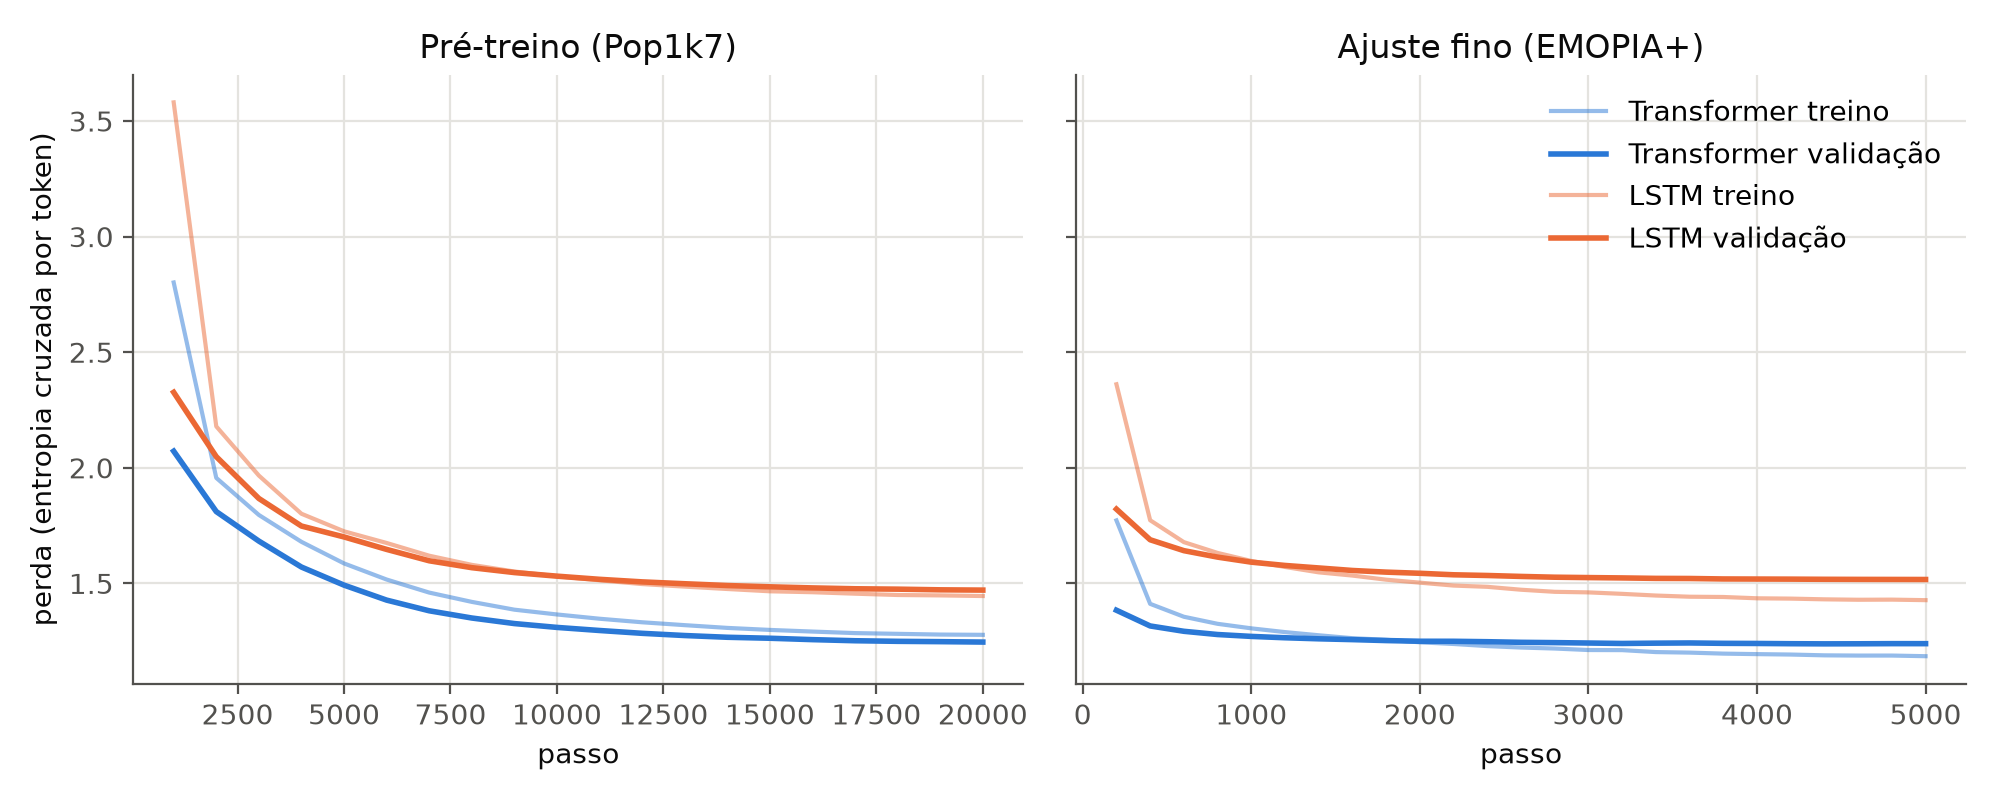
\includegraphics[width=\columnwidth]{fig3_loss_curves}
  \caption{Perda de treino e validação no pré-treino (Pop1k7) e no ajuste fino
    (EMOPIA+).}
  \label{fig:loss}
\end{figure}

\subsection{Aderência e Custo do CFG}

A Tabela~\ref{tab:main} e a Figura~\ref{fig:tradeoff} resumem o efeito de
$\gamma$. Sem CFG, o Transformer acerta o quadrante em apenas 34,0\,\% dos
trechos, abaixo até da LSTM (40,3\,\%). A acurácia cresce quase monotonicamente
com $\gamma$ e chega a 55,7\,\% em $\gamma = 5$ (IC de 51\,\% a 61\,\%), perto
do teto de 58,0\,\%. A diferença para $\gamma = 1$ já é significativa em
$\gamma = 2$ ($p = 0{,}005$) e muito forte em $\gamma = 5$ ($p < 10^{-9}$). A
partir daí o ganho satura: $\gamma = 8$ e $\gamma = 10$ obtêm 55,5\,\% e
58,3\,\%, sem diferença significativa para $\gamma = 5$.

\begin{figure}[t]
  \centering
  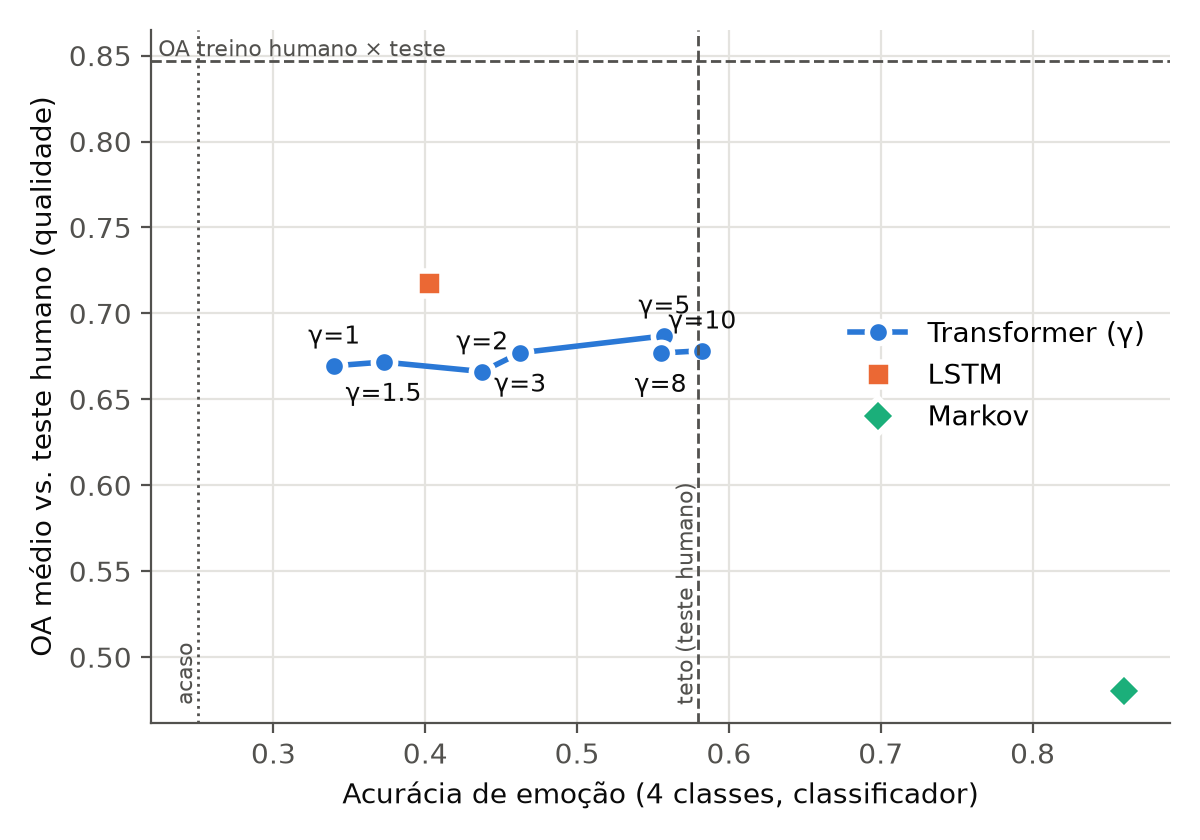
\includegraphics[width=\columnwidth]{fig1_tradeoff}
  \caption{Aderência (acurácia em 4 classes) contra qualidade (OA médio) para
    cada sistema. As linhas tracejadas marcam o teto do classificador e o OA do
    treino humano contra o teste humano.}
  \label{fig:tradeoff}
\end{figure}

Até $\gamma = 5$, esse ganho não tem custo mensurável. O OA médio fica entre
0,666 e 0,687, até subindo um pouco, a diversidade permanece em 0,64 e a
fração de 16-gramas copiados do treino continua em 0,6\,\%, abaixo dos 0,9\,\%
do próprio teste humano. Com CFG, cada quadrante adquire um perfil próprio, mais
próximo do quadrante humano correspondente.

Em $\gamma = 8$ e $\gamma = 10$ surgem sinais leves de degradação. O KL médio
sobe de 0,70 para 1,02, puxado sobretudo pelo \emph{empty beat rate}, cujo OA cai
de 0,68 para 0,48: os quadrantes calmos passam a ter mais tempos vazios do que os
trechos humanos. A taxa de tokens REMI descartados na conversão para MIDI, ainda
pequena, aumenta cerca de 7 vezes (de 0,013\,\% para 0,096\,\%), e a diversidade
cai de 0,640 para 0,623. Como outras métricas, como \emph{scale consistency} e
\emph{polyphony}, melhoram ao mesmo tempo, o OA médio fica estável. O
compromisso entre aderência e qualidade existe, portanto, mas é fraco e só
aparece depois que a aderência já saturou, o que faz de $\gamma \approx 5$ a
melhor escolha.

\subsection{Por que a Valência Não Responde}

A Figura~\ref{fig:va} separa a aderência nos dois eixos. A acurácia de arousal
sobe de 61,5\,\% para 90,5\,\% em $\gamma = 5$ ($p < 10^{-20}$) e chega a
95,5\,\% em $\gamma = 10$, acima do teto humano de 84,1\,\%. A de valência
passa apenas de 56,2\,\% para 61,8\,\%, diferença não significativa
($p = 0{,}11$), e fica sempre abaixo do teto de 69,3\,\%. As matrizes de
confusão mostram o mesmo padrão: em $\gamma = 10$, quase nenhum trecho pedido
como agitado (Q1 ou Q2) é classificado como calmo, e vice-versa, mas 96 dos 100
trechos pedidos como Q1 são classificados como Q2, e os pedidos como Q3 se
dividem entre Q3 (48) e Q4 (36). O acerto em Q1 até cai, de 11\,\% para 4\,\%,
porque o CFG torna esses trechos mais agitados sem torná-los mais alegres. Parte
dessa confusão vem do próprio classificador, que acerta só 32\,\% do Q1 humano,
mas a análise de atributos, que não depende dele, confirma o padrão.

\begin{figure}[t]
  \centering
  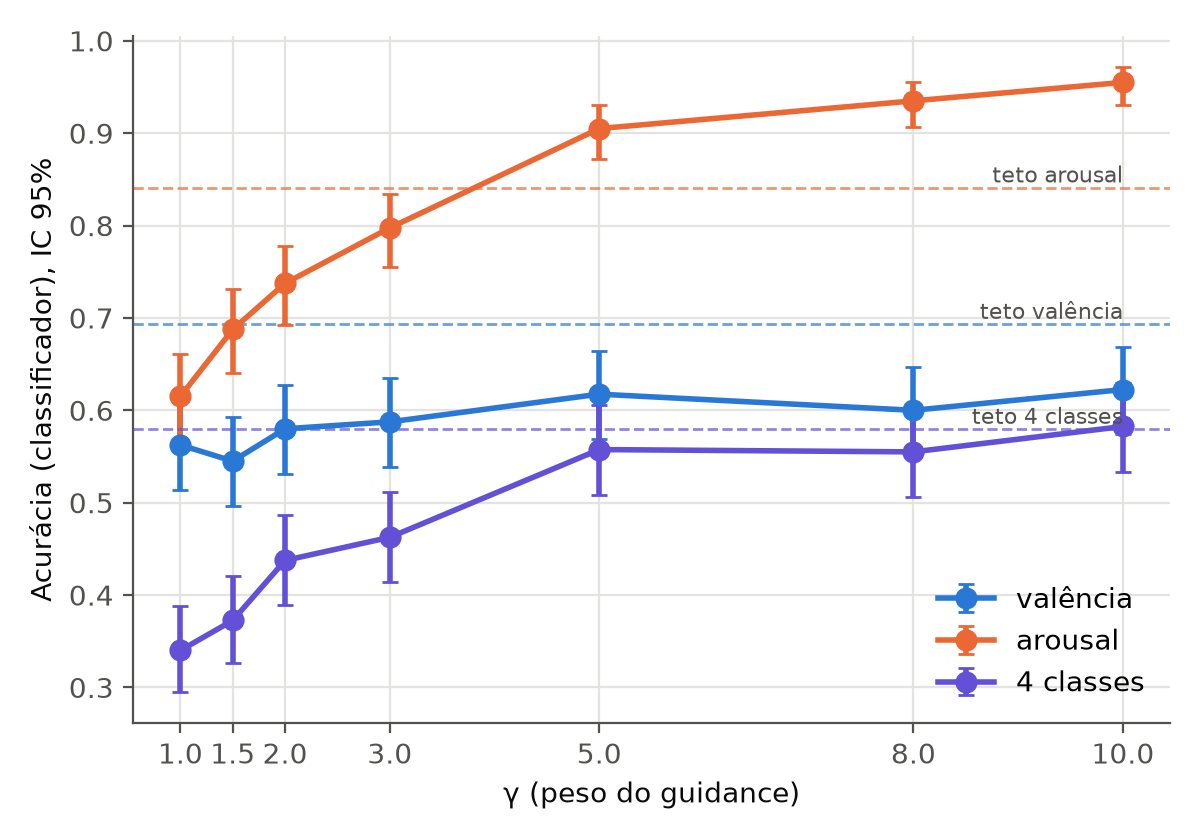
\includegraphics[width=\columnwidth]{fig2_valence_arousal}
  \caption{Acurácia de valência, arousal e 4 classes em função de $\gamma$, com
    IC de 95\,\%. As linhas tracejadas são os tetos medidos no teste humano.}
  \label{fig:va}
\end{figure}

\begin{figure*}[t]
  \centering
  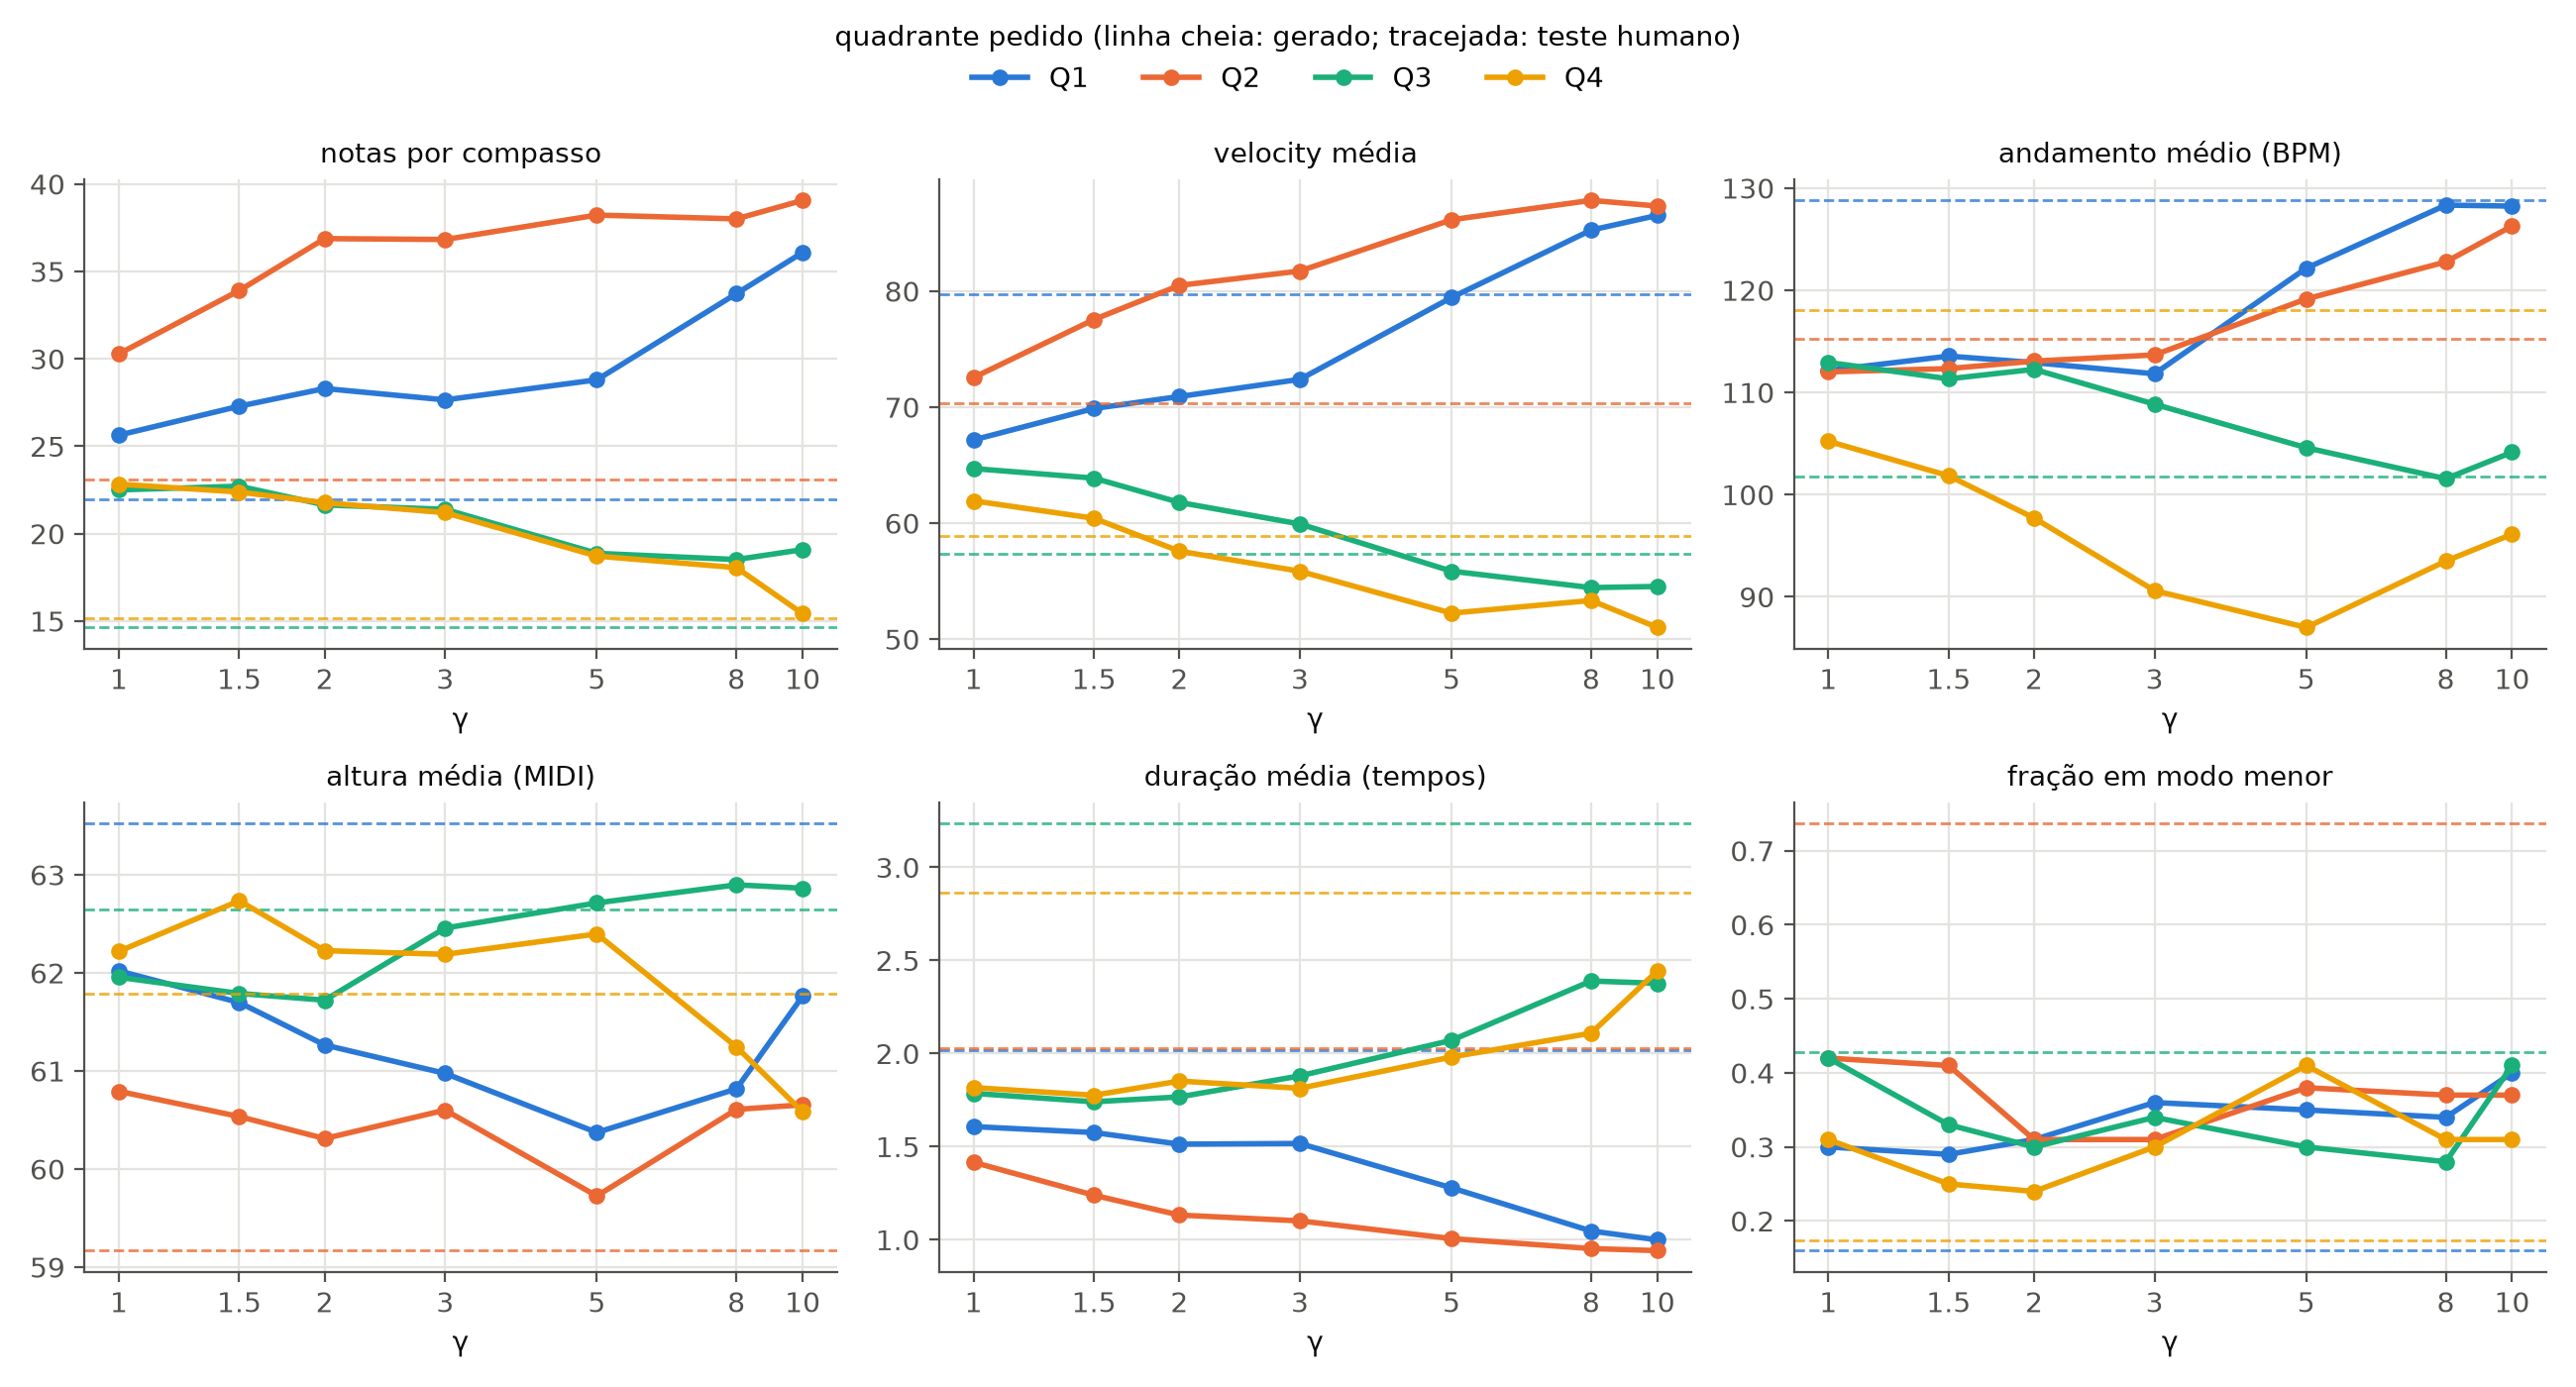
\includegraphics[width=\textwidth]{fig4_attributes}
  \caption{Atributos musicais por quadrante pedido em função de $\gamma$ (linhas
    cheias) e no teste humano (linhas tracejadas). Os atributos ligados ao
    arousal se separam com $\gamma$; a fração em modo menor não.}
  \label{fig:attr}
\end{figure*}

A Figura~\ref{fig:attr} mostra o que o CFG muda na música. Em $\gamma = 1$, os
quatro quadrantes são parecidos, com 23 a 30 notas por compasso,
\emph{velocity} média entre 62 e 73 e andamento entre 105 e 113 BPM. À medida
que $\gamma$ cresce, Q1 e Q2 ficam mais densos, mais fortes, mais rápidos e com
notas mais curtas, e Q3 e Q4 mais esparsos, mais suaves e com notas mais longas.
Em $\gamma = 5$, a \emph{velocity} (80, 86, 56 e 52 de Q1 a Q4) já separa os
quadrantes agitados dos calmos como no teste humano (80, 70, 57 e 59); em $\gamma \geq 8$, os valores ultrapassam os
humanos, e Q2 chega a 39 notas por compasso contra 23 nos trechos reais. Esse
exagero explica a acurácia de arousal acima do teto: o classificador recebe
trechos mais agitados do que qualquer peça real.

A fração em modo menor, por outro lado, não responde ao CFG. No teste humano,
ela separa bem os quadrantes: 0,16 em Q1, 0,74 em Q2, 0,43 em Q3 e 0,17 em Q4.
Nos trechos gerados, fica entre 0,24 e 0,42 em todos os quadrantes e em todos os
valores de $\gamma$, sem tendência. O modelo não aprendeu a associar o modo à
emoção, e o CFG só pode amplificar a diferença entre as predições condicional e
incondicional que o modelo já produz. Esse resultado é coerente com a observação
de que o arousal é mais fácil de capturar a partir de atributos
simbólicos~\cite{Hung2021:emopia} e com a motivação do
EMO-Disentanger~\cite{Huang2024:emodisentanger}, que torna o modo explícito na
representação justamente para controlar a valência. Possíveis causas, não
testadas aqui, são o tamanho reduzido do EMOPIA+, o fato de o modo depender de
relações entre notas ao longo de vários compassos, enquanto densidade e
intensidade aparecem em qualquer trecho local, e a diluição da atenção ao token
de emoção, que aparece só no início da sequência.

\subsection{Comparação com os Baselines}

A LSTM tem a melhor qualidade entre os sistemas gerados (OA de 0,717 e KL de
0,66), um pouco acima do Transformer, apesar da perplexidade pior. As métricas do
MusPy avaliam estatísticas globais, e a LSTM reproduz melhor as distribuições de
altura e de ritmo, enquanto o Transformer gera mais polifonia do que os trechos
humanos (OA de \emph{polyphony} de 0,54). Em aderência, a LSTM supera o
Transformer sem CFG, mas fica bem abaixo dele com $\gamma \geq 2$.

A cadeia de Markov obtém a maior aderência de todas, 86,0\,\% em 4 classes, acima
do teto humano, e a pior qualidade, com OA de 0,480. Como cada quadrante tem a
sua própria cadeia, os atributos locais reproduzem quase exatamente os do
quadrante: Q1 tem 21 notas por compasso contra 22 no humano, e Q3 tem 14 contra
15. O classificador se apoia nesses traços, mas as peças misturam escalas
incompatíveis (OA de 0,13 em \emph{pitch class entropy} e de 0,11 em
\emph{scale consistency}), têm a menor diversidade (0,233) e copiam o treino:
6,6\,\% dos 16-gramas vêm do EMOPIA+, com cópias contínuas de até 72 tokens,
enquanto nenhum trecho do Transformer passa de 24 tokens copiados. O Markov
mostra, de forma extrema, que a aderência medida por um classificador precisa
ser lida junto com a qualidade, e o mesmo cuidado vale para o arousal acima do
teto obtido com $\gamma$ alto.

\subsection{Análise Qualitativa}

\begin{figure}[t]
  \centering
  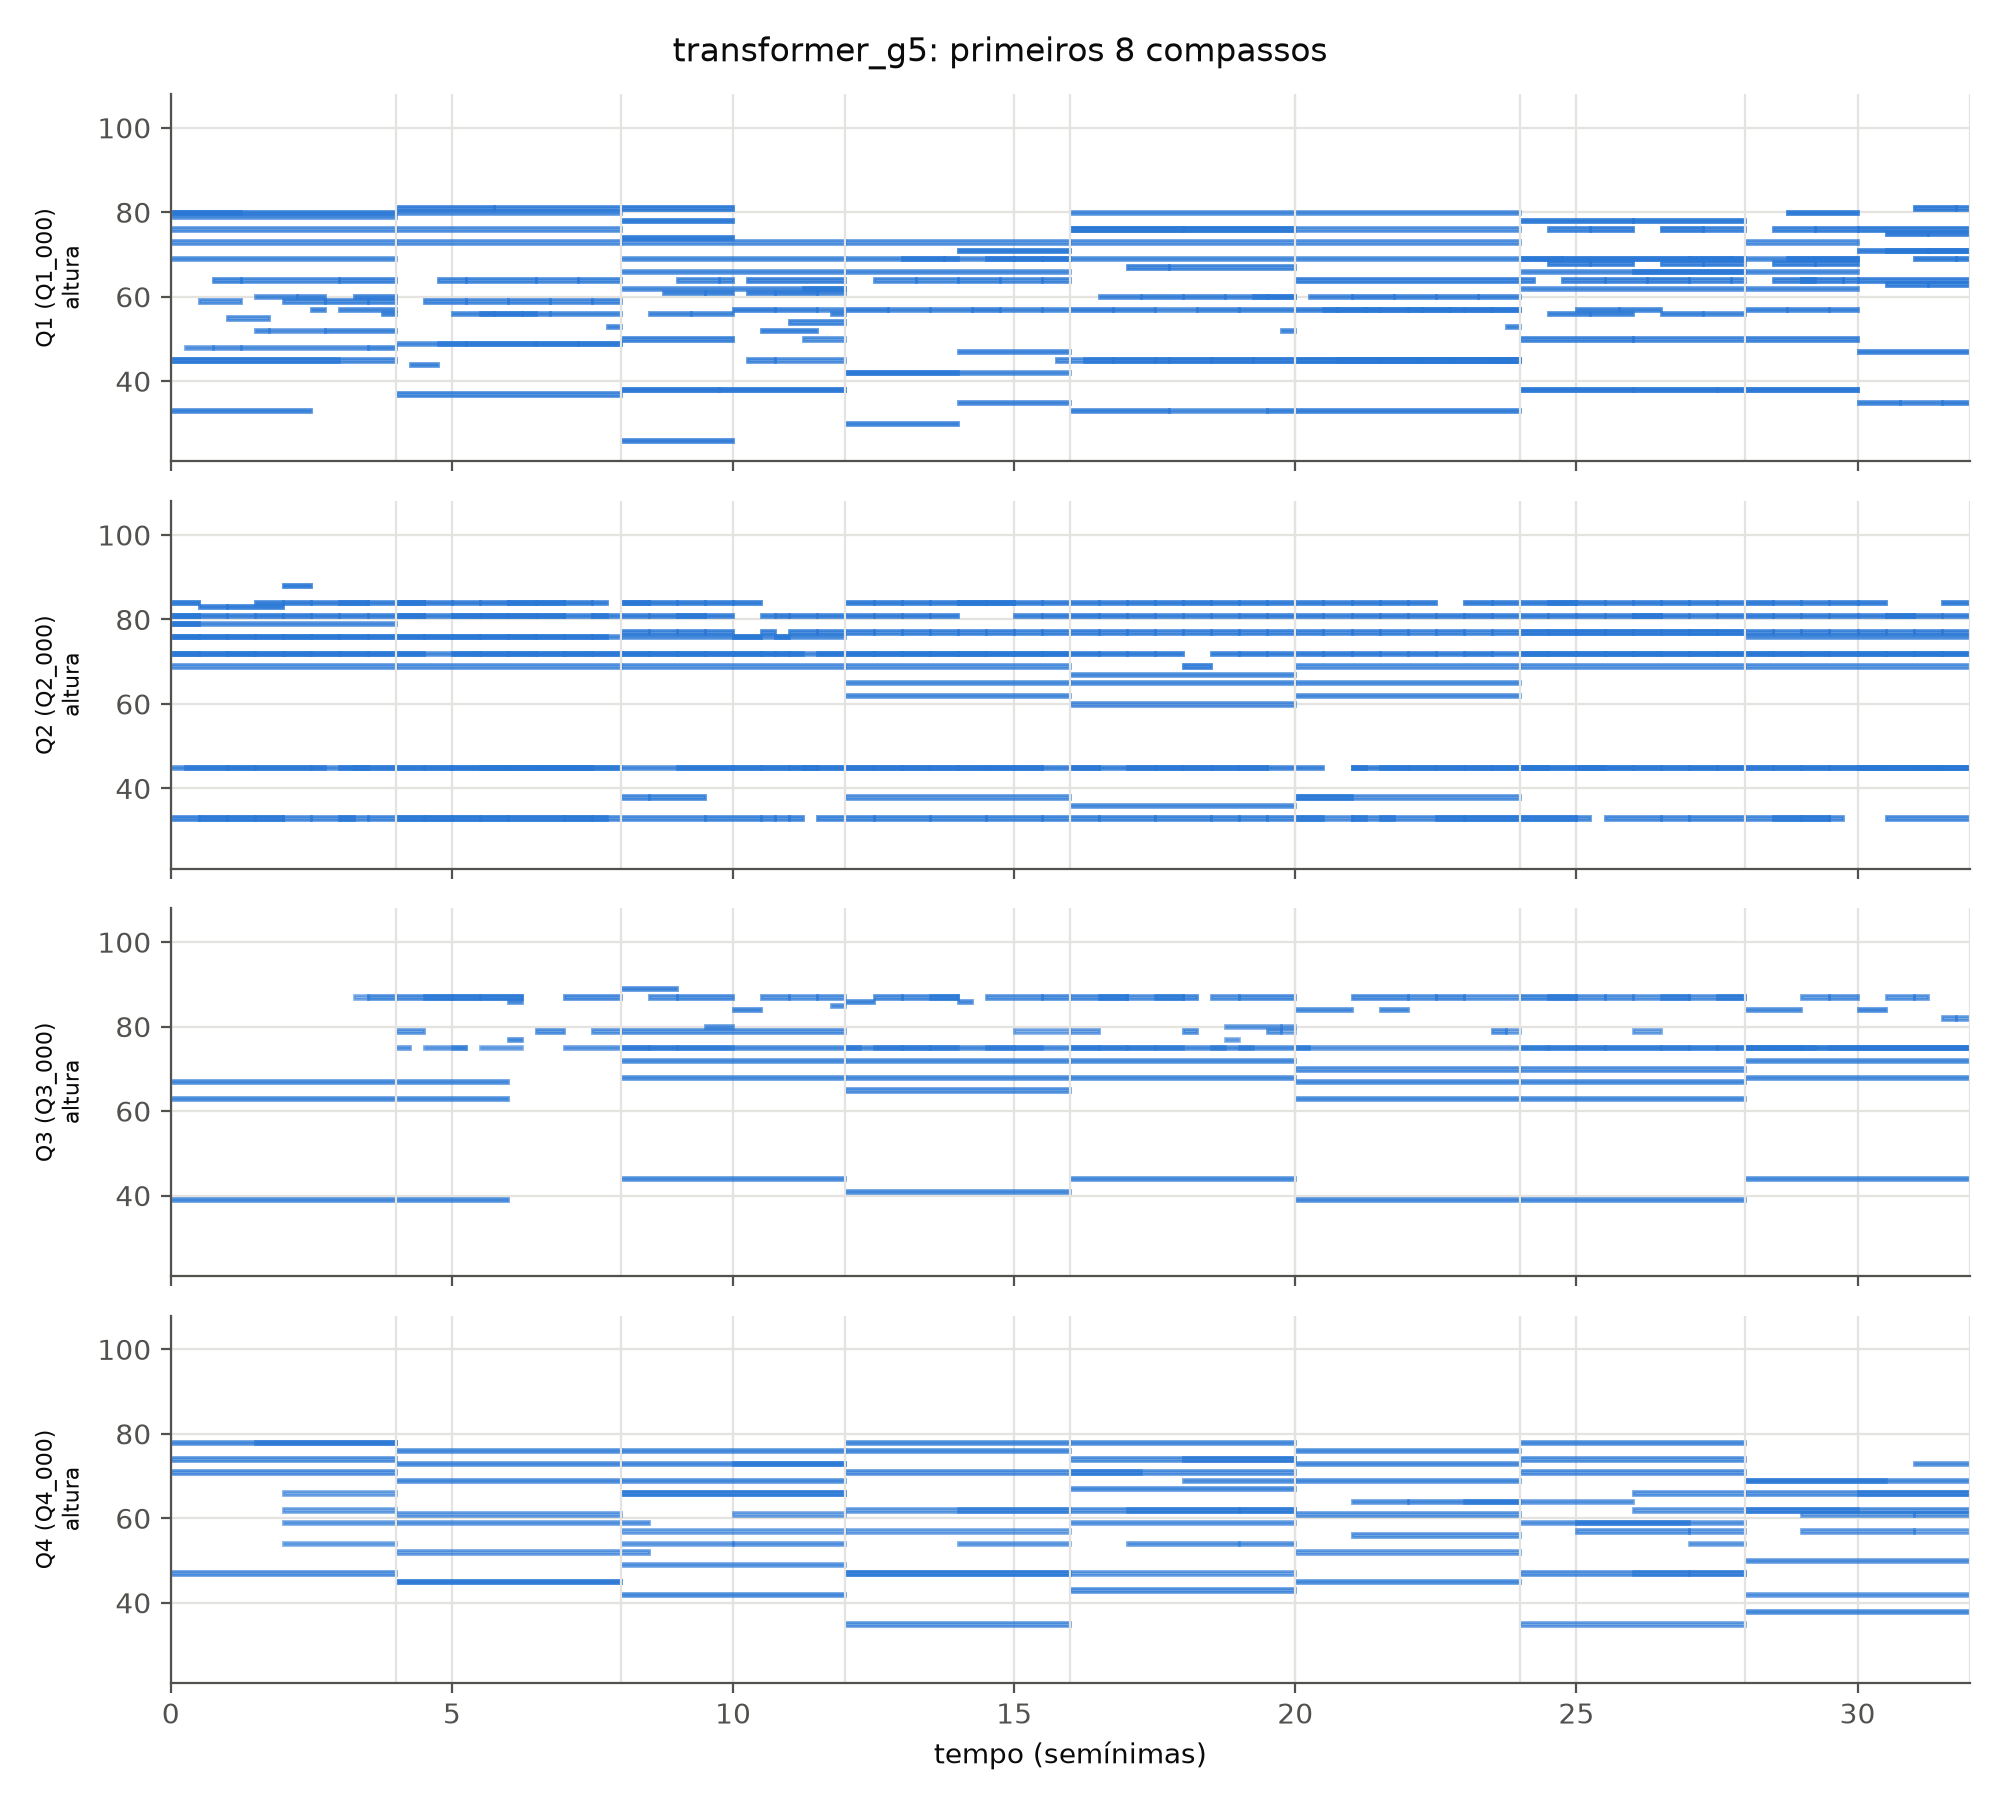
\includegraphics[width=\columnwidth]{pianoroll_transformer_g5}
  \caption{Primeiros 8 compassos do primeiro trecho gerado para cada quadrante,
    com $\gamma = 5$.}
  \label{fig:roll}
\end{figure}

A Figura~\ref{fig:roll} mostra o primeiro trecho gerado para cada quadrante com
$\gamma = 5$, sem seleção manual. O trecho de Q2 tem notas agudas repetidas sobre
um baixo insistente, um padrão denso e obstinado, enquanto o de Q3 começa
esparso, com acordes longos, e só depois ganha uma linha aguda. Q1 tem textura
cheia e movimento na região média, e Q4 é uma sequência de acordes sustentados
que mudam a cada compasso, como em uma balada. Os quadrantes são distintos em
densidade e duração, mas não em harmonia: Q1 não soa claramente mais maior que
Q2, o que é coerente com a análise de modo. Os áudios de dois trechos por
quadrante de cada sistema e do teste humano, sintetizados com FluidSynth e o
\emph{soundfont} MuseScore General, estão no repositório do projeto, em
\texttt{samples/audio}.

% -----------------------------------------------
\section{Conclusão e Trabalhos Futuros}\label{sec:conclusion}

Este trabalho mostrou que o \emph{classifier-free guidance}, aplicado apenas na
amostragem, reforça o condicionamento por emoção em um Transformer de piano pop.
Com $\gamma = 5$, a acurácia em 4 classes sobe de 34\,\% para 56\,\%, perto do
teto do classificador, sem custo de qualidade, diversidade ou memorização; com
valores maiores, a aderência satura e surgem sinais leves de degradação. O ganho,
no entanto, vem quase todo do arousal. A análise de atributos mostra que o CFG
amplifica densidade, intensidade, andamento e duração das notas, mas não altera
o modo, que no modelo não se associa à emoção. O CFG reforça o que o modelo já
aprendeu, mas não supre o que ele não aprendeu.

O estudo tem limitações. A aderência é medida por um classificador que acerta
58\,\% no teste humano, com apenas 88 trechos, e tanto a cadeia de Markov quanto o
CFG com $\gamma$ alto mostram que um gerador pode explorar os traços em que o
classificador se apoia. Os modelos foram treinados com uma única semente. Como trabalhos futuros, propõe-se um teste de audição com modelo,
baselines e peças humanas, para verificar se a emoção percebida acompanha o
classificador; condicionar explicitamente a tonalidade ou o modo, como no
EMO-Disentanger~\cite{Huang2024:emodisentanger}; usar pesos de \emph{guidance}
separados para valência e arousal; e repetir o token de emoção ao longo da
sequência para reduzir a diluição da condição.

% -----------------------------------------------
\bibliography{ISMIRtemplate}

\end{document}
